\chapter{Background concepts}

\label{chapter:background}

\section{Explainable artificial intelligence}

\label{section:xai}

In this section, we lay out background concepts for Explainable Artificial Intelligence (XAI) which have been largely adopted from \citet{arrieta2020explainable}. The study is particularly helpful for us since it summarizes the findings of approximately 400 XAI contributions and presents these findings in the form of well-defined concepts and taxonomies. In addition, the study discusses future directions of XAI research. We start off by providing definitions from the study, along with accompanying remarks.

\subsection{Transparency}

\begin{definition}[Transparency; \citealt{arrieta2020explainable}]
  A model is considered to be transparent if it is understandable on its own without any external techniques to assist its understandability. Since a model can provide different degrees of understandability, transparent models are split into three possibly mutually-inclusive categories; specifically simulatable models, decomposable models and algorithmically transparent models. 
\end{definition}

\begin{remark}
  \textit{Simulatability} refers to the ability of a model's inner-mechanisms being simulated strictly by a human. Therefore, model simplicity plays a major role in this class.
\end{remark}

\begin{remark}
  \textit{Decomposability} refers to the ability to clearly understand the individual parts of a model; such as its inputs, parameters and basic computational mechanisms.
\end{remark}

\begin{remark}
  \textit{Algorithmic transparency} refers to the ability of a human to understand the algorithmic processes used in the model to produce any given output from any given input.
\end{remark}

\begin{remark}
  A model is considered transparent if it falls into one or more of the aforementioned transparency categories. If a model cannot satisfy any of the requirements of being transparent, then it is classified as a \textit{black-box} model. 
\end{remark}

\begin{remark}
  \label{rmk:equivalence}
  As recommended by \citet[Section 2.1, Page 3]{arrieta2020explainable}, we use the terms transparency and interpretability to refer to the same feature. Therefore, we use these terms equivalently and interchangeably.
\end{remark}

Examples of well-known transparent Machine Learning (ML) models are linear/logistic regressors, decision trees and rules-based learners. Similarly, common examples of black-box ML models are tree ensembles and deep neural networks. \citet{arrieta2020explainable} provide extensive justifications using the aforementioned three criteria in conducting model classifications into the transparent and black-box categories. We would direct the reader to their study for a full analysis and justification of these classifications.

\subsection{Explainability and XAI}

\begin{definition}[Explainability; \citealt{arrieta2020explainable}]
  Explainability refers to the interface between humans and a model, such that this interface is both an accurate proxy of the model and comprehensible to humans. 
\end{definition}

\begin{definition}[Explainable Artificial Intelligence; \citealt{arrieta2020explainable}]
  An explainable artificial intelligence is one that produces details to make its functioning understandable to a given target audience. 
\end{definition}

\citet{arrieta2020explainable} observe that black-box ML models are increasingly being employed to make important predictions in critical contexts, citing high-risk areas such as precision medicine and autonomous vehicles. Of particular relevance to the field of Natural Language Processing (NLP), the study notes a myriad of issues related to inductive biases within training data sets and the ethical issues involved in using black-box models trained on such data sets. As a result, they describe an increased demand for transparency in black-box ML models from the various stakeholders in Artificial Intelligence (AI). In addition, \citet{arrieta2020explainable} emphasize the presence of a target audience for XAI; implying that different XAI techniques should be employed for different target audiences. In their study, they provide examples of target audiences such as domain experts, end-users and managers (Figure \ref{fig:xai-target-audience}).

\begin{figure}[t]
  \centering
  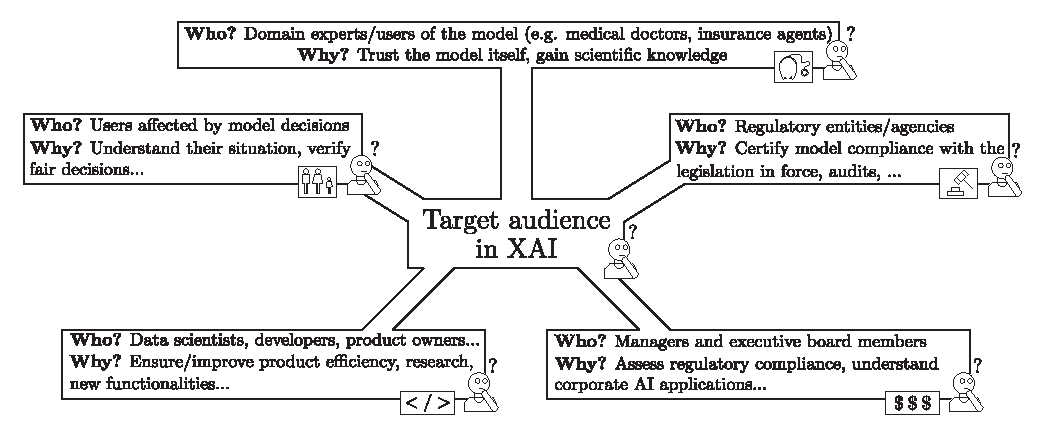
\includegraphics[trim={0.1cm 0.1cm 0.1cm 0.1cm},clip,width=14cm]{pdfs/xai_target_audience}
  \caption{Examples of various target audiences in XAI; figure taken from \citet{arrieta2020explainable}}
  \label{fig:xai-target-audience}
\end{figure}

\subsection{Terminology clarification}

\label{section:xai-terminology}

Based on an extensive literature review, \citet{arrieta2020explainable} observe that many studies tend to misuse the terms interpretability and explainability by using them interchangeably. To address this, they provide clear conceptual differences between the terms. For example, \citet[Section 2.1, Page 3]{arrieta2020explainable} state that \textit{``interpretability refers to a passive characteristic of a model referring to the level at which a given model makes sense for a human observer.''} In contrast, \citet[Section 2.1, Page 3]{arrieta2020explainable} state that \textit{``explainability can be viewed as an active characteristic of a model, denoting any action or procedure taken by a model with the intent of clarifying or detailing its internal functions.''}

In summary, we gather that interpretability (or transparency as per Remark \ref{rmk:equivalence}) refers to an inherent or passive feature of a model. On the other hand, explainability refers to an active characteristic undertaken by the model and its developers to explain the model's inner mechanisms. In addition, explainability entails the presence of a target audience; which may not necessarily be the case for interpretability or transparency.

\subsection{Explainability techniques}

\label{section:xai-techniques}

Based on the aforementioned classification of ML models into transparent and black-box models, \citet{arrieta2020explainable} expound on explainability techniques for each of these model types. Due to their transparent nature, the study states that transparent ML models are usually explainable in themselves to most target audiences and therefore usually do not require any external technique to extract explanations. The study does however highlight some target audiences, such as non-expert users, who may require external explainability techniques such as model output visualizations in order to explain the inner workings of transparent ML models.

For the case of black-box models, \citet{arrieta2020explainable} argue that separate or external techniques must be utilized in order to reasonably explain these models. Such explainability techniques are referred to in the study as post-hoc explainability techniques; which is derived from the idea that explanations for such models are usually extracted post-modeling. Notable examples of post-hoc explainability techniques include local explanations, feature relevance and explanations by simplification.

\begin{definition}[Local explanations; \citealt{arrieta2020explainable}]
  Local explanations operate by segmenting a model's solution space into subspaces and provide explanations for the less complex model subspaces.
\end{definition}

\begin{remark}
  Local explanations are commonly used in XAI research and function by using differentiating properties on model solution space subsets.
\end{remark}

\begin{remark}
  Two well-known examples of local explainability techniques are Local Interpretable Model-Agnostic Explanations (LIME; \citealt{lime}) and G-REX \citep{konig2008g}.
\end{remark}

\begin{definition}[Feature relevance; \citealt{arrieta2020explainable}]
  Feature relevance explanation methods operate by computing an importance score for the model's input variables over the model's output variables. These scores typically quantify how sensitive the model's output is to perturbations in the model's inputs.
\end{definition}

\begin{remark}
  Feature relevance methods can be considered as indirect methods of explaining a model. 
\end{remark}

\begin{remark}
  Well-known feature relevance explainability techniques include the Shapley Additive Explanations (SHAP; \citealt{lundberg2017unified}) and the occlusion sensitivity method \citep{zeiler2014visualizing}.
\end{remark}

\begin{definition}[Explanations by simplification; \citealt{arrieta2020explainable}]
  Explanations by simplification refer to techniques where a simplified proxy model is built to approximate and explain a more complex model. The simplified proxy model usually has to fulfil the the joint criteria of reducing its complexity compared to its antecedent model while maximizing its resemblance to its antecedent and keeping a similar performance score.
\end{definition}

\begin{remark}
  In this thesis, we refer to the original black-box model as an \textit{antecedent} model and the simplified model as the \textit{proxy} model. Furthermore, we qualify that all proxy models must be designed to globally approximate their respective antecedent models.
\end{remark}

\begin{remark}
  \citet{bastani2017interpretability} and \citet{tan2018distill} are examples of studies that extract and distill simpler proxy models from complex antecedent models.
\end{remark}

Through a survey of recent literature on explanations by simplification applied in the Natural Language Processing (NLP) field, we came across several prominent studies employing explanations by simplification to simplify antecedent black-box neural networks into proxy Finite-State Automata (FSAs) and/or Weighted Finite-State Automata (WFSAs) \citep{schwartz2018sopa,peng2018rational,DBLP:journals/corr/abs-1905-08701,wang2019state,jiang2020cold}. We expound more on WFSAs and \citet{schwartz2018sopa} in Sections \ref{section:wfsa} and \ref{section:soft-patterns} respectively.

\begin{figure}[t]
  \centering
  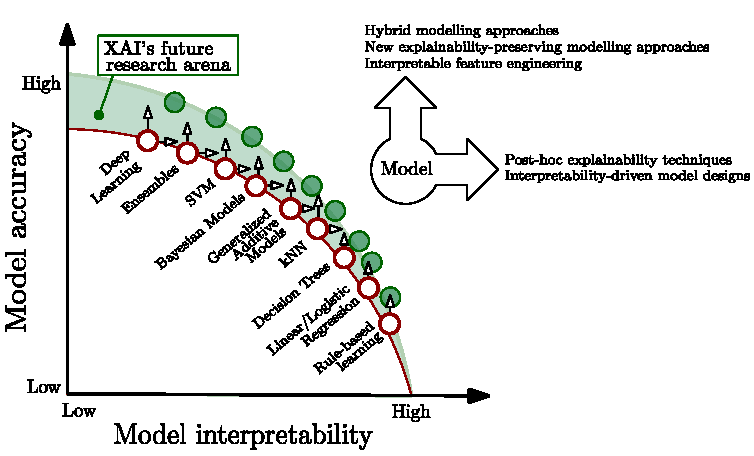
\includegraphics[width=14cm]{pdfs/performance_transparency_tradeoff.pdf}
  \caption{Schematic visualizing the performance-interpretability tradeoff; figure taken from \citet{arrieta2020explainable}}
  \label{fig:performance_interpretability_tradeoff}
\end{figure}

\subsection{Performance-interpretability tradeoff}

An interesting and insightful contribution of \citet[Section 5.1, Page 18]{arrieta2020explainable} is the description of the performance-interpretability tradeoff; which they cautiously introduce as \textit{``the matter of interpretability versus performance is one that repeats itself through time, but as any other big statement, has its surroundings filled with myths and misconceptions.''} To address some of the aforementioned myths and misconceptions, \citet{arrieta2020explainable} first disprove the generic statement that more complex models are always more accurate by pointing to certain case studies to support this argument. In particular, they show that complex models are not necessarily more accurate in cases where the function to be modeled is not complex, data is well-structured and input features are available with high quality.

Next, \citet{arrieta2020explainable} provide the case where the aforementioned statement, that complex models perform better, tends to be true. According to the study, this is usually true when the function to be modeled is sufficiently complex and where the input data has high diversity or variance; and possibly contains significant noise. In such cases, \citet{arrieta2020explainable} argue that the performance-interpretability tradeoff can be observed; as exemplified in Figure \ref{fig:performance_interpretability_tradeoff}.
 
\subsection{Explainability metrics}

\label{section:xai-metrics}

Towards the end of their study, \citet{arrieta2020explainable} note two major limitations of the current state of XAI research. Firstly, they observe the lack of a unified conceptualization of explainability between various studies. They furthermore acknowledge that their study, while limited, could provide a good starting point for other XAI studies. Secondly, \citet{arrieta2020explainable} note the lack of a unified metric that denotes how explainable any given model is. They further explain why developing such a metric has been a difficult process for many XAI studies; particularly because such a metric would entail incorporating psychological, sociological and cognitive elements to accommodate the goodness of fit of an explainability method to a certain target audience. Furthermore, incorporating such elements might involve significant amounts of subjectivity in the desired metric.

To reduce some of the aforementioned subjectivity involved, \citet{MILLER20191} and \citet{arrieta2020explainable}  provide basic guidelines of what could constitute a good explanation based on human psychology, sociology and cognitive sciences. Firstly, they observe that explanations are better when \textit{constrictive}; meaning an explanation is good if it not only explains why a model made decision X, but also why it made decision X over decision Y. Next, they suggest that good explanations should be able to communicate causal links over probabilities; which could be a challenge for black-box models which generally compute aggregate probabilities without necessarily considering causal links. Finally, they recommend that explanations are better when \textit{selective}; meaning that a good explanation should be able to selectively provide the most important causal links instead of all possible causal links as these might be irrelevant or confusing to the target audience.

\section{Straight-through estimator}

Activation quantized neural networks refer to neural networks that contain layers which transmit piece-wise discrete signals. One of the main challenges in training such activation quantized neural networks is that their gradients tend to vanish almost everywhere because their derivatives typically default to zero. \citep{bengio2013estimating,courbariaux2016binarized,yin2019understanding}.

One significant workaround for this issue was proposed by \citet{bengio2013estimating} through the introduction of the Straight-Through Estimator (STE). In the vanilla version of the STE, the STE neuron emits a signal of 1 when its input is strictly positive, and emits a zero signal in all other cases (Equation \ref{eq:ste-forward}). The STE then uses a simple identity function to estimate the gradient during the backward pass (Equation \ref{eq:ste-backward}). The vanilla STE is visualized through a schematic in Figure \ref{fig:straight-through-estimator}.

\begin{equation}
  \label{eq:ste-forward}
  \text{STE}(x)=
  \begin{cases}
    1 & x > 0 \\
    0 & x \leq 0
  \end{cases}
\end{equation}

\begin{equation}
  \label{eq:ste-backward}
  \text{STE}'(x)= x
\end{equation}

\begin{figure}[t]
  \centering
  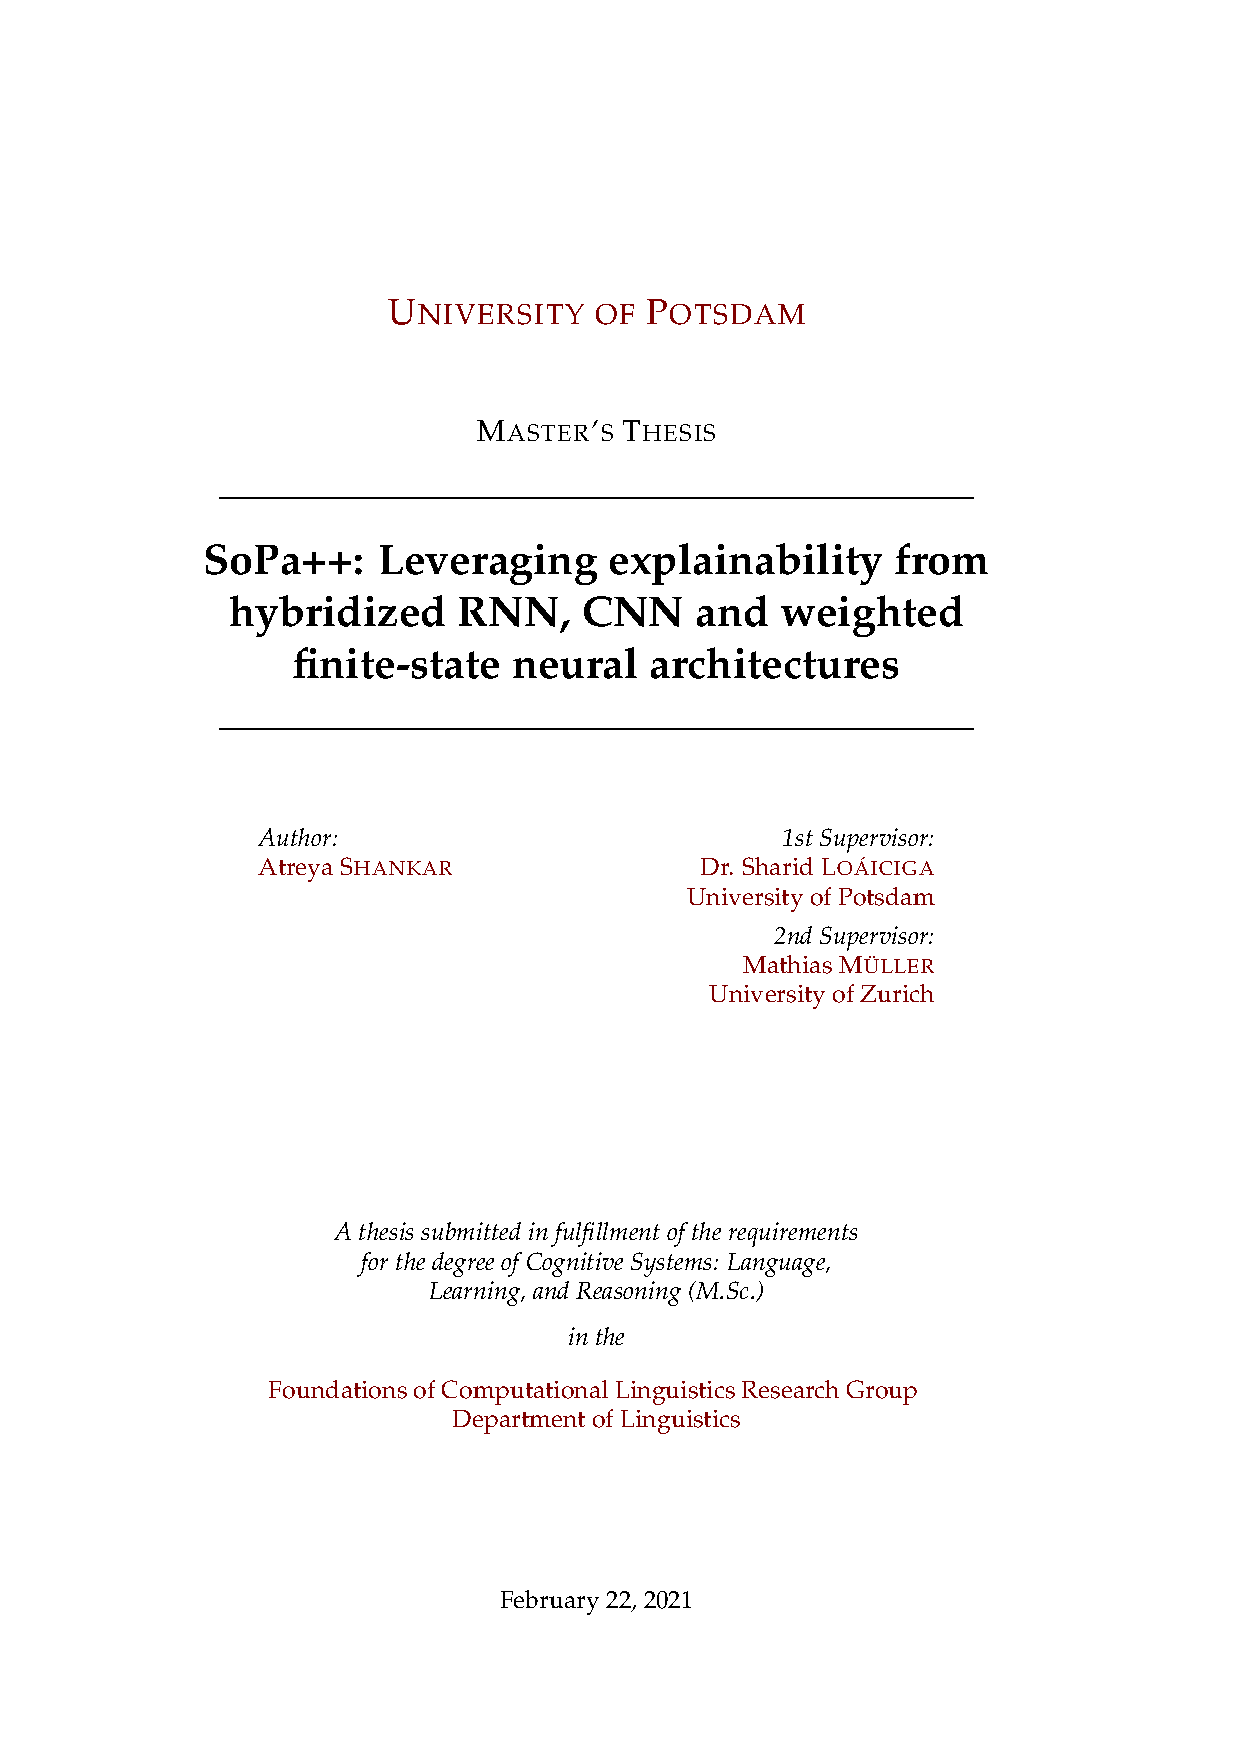
\includegraphics[width=14cm]{pdfs/ste_theoretical/main.pdf}
  \caption{Schematic visualizing the vanilla STE's forward and backward passes}
  \label{fig:straight-through-estimator}
\end{figure}

Aside from the vanilla STE, several other flavors of STEs have been proposed by studies such as \citet{courbariaux2016binarized} and \citet{yin2019understanding}. In general, these studies have shown that activation quantized neural networks perform competitively with their non-quantized counterparts; while providing performance-related benefits related to lower precision computing as well as enabling further research into threshold driven neural activation functions.

\section{Weighted finite-state automaton}

\label{section:wfsa}

\begin{definition}[Semiring; \citealt{kuich1986linear}]
  A semiring is a set $\mathbb{K}$ along with two binary associative operations $\oplus$ (addition) and $\otimes$ (multiplication) and two identity elements: $\bar{0}$ for addition and $\bar{1}$ for multiplication. Semirings require that addition is commutative, multiplication distributes over addition, and that multiplication by $\bar{0}$ annihilates, i.e., $\bar{0} \otimes a = a \otimes \bar{0} = \bar{0}$.

\begin{remark}
  Semirings follow the following generic notation: $\langle \mathbb{K}, \oplus, \otimes, \bar{0}, \bar{1} \rangle$.
\end{remark}

\begin{remark}
  A simple and common semiring is the real or sum-product semiring: $\langle \mathbb{R}, +, \times, 0, 1 \rangle$. Two important semirings for this thesis are shown below.
\end{remark}

\begin{remark}
  \textbf{Max-sum} semiring: $\langle \mathbb{R} \cup \{-\infty\}, \text{max}, +, -\infty, 0 \rangle$
\end{remark}

\begin{remark}
  \textbf{Max-product} semiring: $\langle \mathbb{R}_{>0} \cup \{-\infty\}, \text{max}, \times, -\infty, 1 \rangle$
\end{remark}

\end{definition}

\begin{definition}[Weighted finite-state automaton; \citealt{peng2018rational}]
  \label{def:wfsa}
  A weighted finite-state automaton over a semiring $\mathbb{K}$ is a 5-tuple $\mathcal{A} = \langle \Sigma, \mathcal{Q}, \mathcal{T}, \lambda, \rho \rangle$, with:

  \begin{itemize}
    \itemsep0em 
    \item[--] a finite input alphabet $\Sigma$;
    \item[--] a finite state set $\mathcal{Q}$;
    \item[--] transition weights $\mathcal{T}: \mathcal{Q} \times \mathcal{Q} \times (\Sigma \cup \{\epsilon\}) \rightarrow \mathbb{K}$;
    \item[--] initial weights $\lambda: \mathcal{Q} \rightarrow \mathbb{K}$; 
    \item[--] and final weights $\rho: \mathcal{Q} \rightarrow \mathbb{K}$.
  \end{itemize}

  \begin{remark}
    Several studies refer to the transition weights $\mathcal{T}$ as the transition matrix, and the initial $\lambda$ and final $\rho$ weights as the initial and final weight vectors respectively \citep{schwartz2018sopa,jiang2020cold}. As a result, we may use these terms interchangeably when referring to different studies.
  \end{remark}
  
  \begin{remark}
    $\epsilon \notin \Sigma$ refers to special $\epsilon$-transitions that may be taken without consuming any input.
  \end{remark}

  \begin{remark}
    Self-loop transitions in $\mathcal{A}$ refer to special transitions which consume an input while staying at the same state.
  \end{remark}
  
  \begin{remark}
    $\Sigma^{*}$ refers to the (possibly infinite) set of all strings over the alphabet $\Sigma$.
  \end{remark}
   
\end{definition}

\begin{definition}[Path score; \citealt{peng2018rational}]

  Let $\pmb{\pi} = \langle \pi_1, \pi_2, \dots, \pi_n \rangle$ be a sequence of adjacent transitions in $\mathcal{A}$, with each $\pi_i = \langle q_i, q_{i+1}, z_i \rangle \in \mathcal{Q} \times \mathcal{Q} \times (\Sigma \cup \{\epsilon\})$. The path $\pmb{\pi}$ derives the $\epsilon$-free string $\pmb{x} = \langle x_1, x_2, \dots, x_m \rangle \in \Sigma^{*}$; which is a substring of the $\epsilon$-containing string $\pmb{z} = \langle z_1, z_2, \dots, z_n \rangle \in (\Sigma \cup \{\epsilon\})^{*}$. $\pmb{\pi}$'s score in $\mathcal{A}$ is given by:
  
\end{definition}

\begin{equation}
  \mathcal{A}[\pmb{\pi}] = \lambda(q_1) \otimes \Bigg( \bigotimes_{i=1}^n \mathcal{T}(\pi_i) \Bigg) \otimes \rho(q_{n+1})
\end{equation}

\begin{definition}[String score; \citealt{peng2018rational}]
\label{def:string-score}
Let $\Pi(\pmb{x})$ denote the set of all paths in $\mathcal{A}$ that derive $\pmb{x}$. Then the string score assigned by $\mathcal{A}$ to string $\pmb{x}$ is given by:
  
\end{definition}

\begin{equation}
  \mathcal{A}[\![\pmb{x}]\!] = \bigoplus_{\pmb{\pi} \in \Pi(\pmb{x})} \mathcal{A}[\pmb{\pi}]
\end{equation}

\begin{remark}
  Since $\mathbb{K}$ is a semiring, $\mathcal{A}[\![\pmb{x}]\!]$ can be efficiently computed using the Forward algorithm \citep{baum1966statistical}. Its dynamic program is summarized below without $\epsilon$-transitions for simplicity. $\Omega_i(q)$ gives the aggregate score of all paths that derive the substring $\langle x_1, x_2, \dots, x_i \rangle$ and end in state $q$:
 
\begin{subequations}
  \begin{align}
    \Omega_0(q) &= \lambda(q) \\
    \Omega_{i+1}(q) &= \bigoplus_{q' \in \mathcal{Q}} \Omega_i(q') \otimes \mathcal{T}(q',q,x_i)  \\
    \mathcal{A}[\![\pmb{x}]\!] &= \bigoplus_{q \in \mathcal{Q}} \Omega_n(q) \otimes \rho(q)
  \end{align}
\end{subequations}

\end{remark}

\begin{remark}
  \label{rmk:old-runtime}
  The Forward algorithm can be generalized to any semiring \citep{eisner2002parameter} and has a runtime of $O(|Q|^3 + |Q|^2|\pmb{x}|)$ \citep{schwartz2018sopa}; notably with a linear runtime with respect to the length of the input string $\pmb{x}$.
\end{remark}

\begin{remark}
  A special case of Forward is the Viterbi algorithm, where the addition $\oplus$ operator is constrained to the maximum function \citep{viterbi1967error}. Viterbi therefore returns the highest scoring path $\pmb{\pi}$ that derives the input string $\pmb{x}$.
\end{remark}

\section{Soft patterns}

\label{section:soft-patterns}

\citet{schwartz2018sopa} present a novel hybridized RNN, CNN and WFSA-based neural architecture called \textbf{So}ft \textbf{Pa}tterns (SoPa). This architecture resembles a RNN because it processes text sequentially and can encode strings of arbitrary lengths. Similarly, the architecture contains a variable number of constrained linear-chain WFSAs with variable pattern lengths or window sizes; which resembles both one-layer CNNs and an ensemble of constrained linear-chain WFSAs. The combination of the aforementioned neural features allows SoPa to learn soft versions of traditional textual surface patterns.

In their study, \citet{schwartz2018sopa} test the SoPa architecture on three separate sentiment classification tasks and compare the results with four baselines which included a bidirectional LSTM and a CNN. With their results, they show that SoPa performed on par or better than all baselines on all tasks. Additionally, they show that SoPa outperformed all baselines significantly in low-data settings. Finally, the authors present a simple method to explain the SoPa model using both local explanations and feature relevance.

\begin{figure}[t]
  \centering
  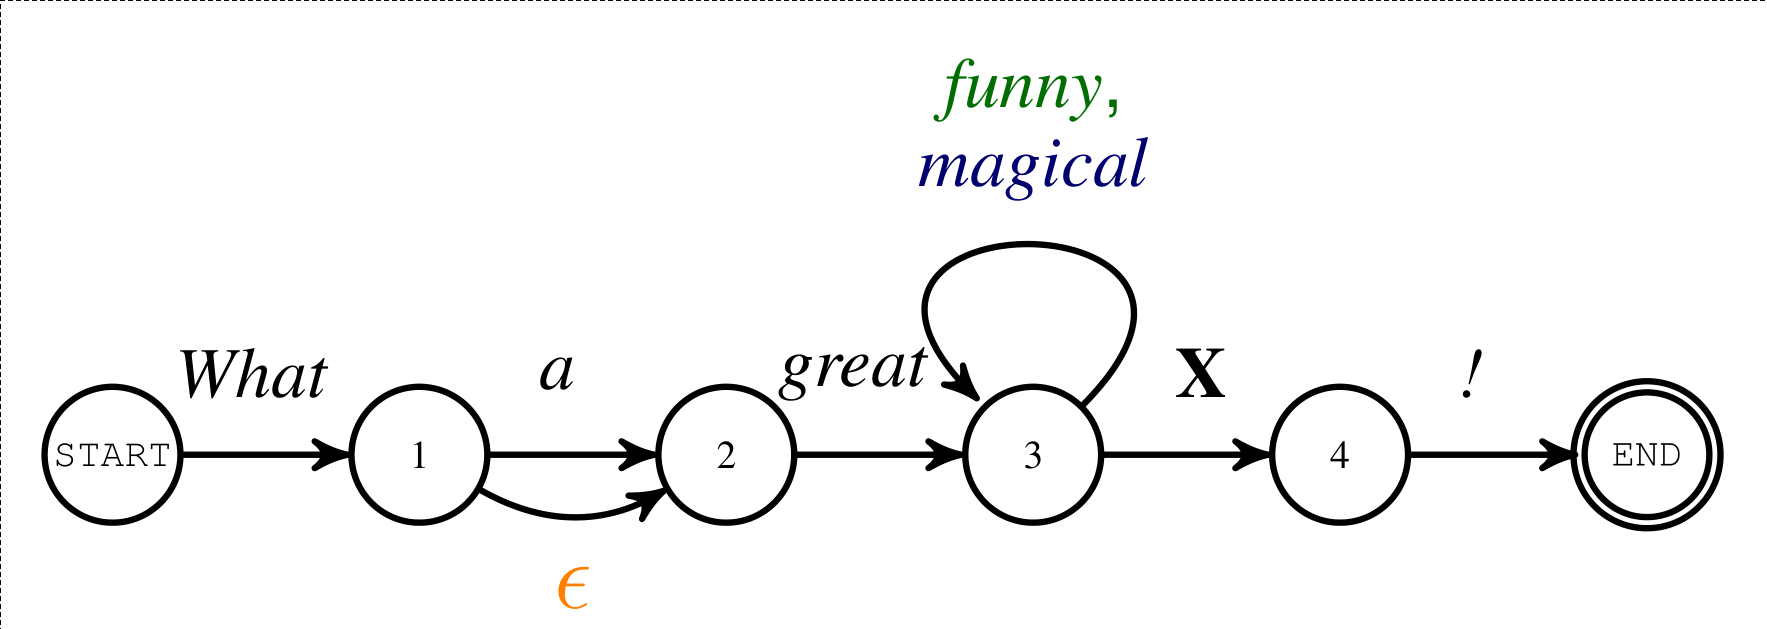
\includegraphics[trim={0.5cm 0.5cm 0.5cm 0.5cm},clip,width=12cm]{images/sample_fsa_sopa.png}
  \caption{Schematic visualizing a linear-chain (weighted) finite-state automaton with one start and end state, $\epsilon$-transitions, self-loops and a wildcard transition shown as \textbf{X}; note that wildcard transitions are not allowed in the SoPa model; figure taken from \citet{schwartz2018sopa}}
  \label{fig:fsa}
\end{figure}

\subsection{Model specifications}

\paragraph{WFSAs:} In regards to the WFSAs used in SoPa, \citet{schwartz2018sopa} only utilize the max-sum and max-product semirings; as well as $\epsilon$-transitions and self-loops. Next, they employ constraints on the model's WFSAs in order to reduce the runtime of SoPa further. Of these, they firstly only allow one start and end state; which results in the initial $\lambda$ and final $\rho$ weights being reduced to static unitary values instead of state-dependent weights found in Definition \ref{def:wfsa}. Next, they constrain $\epsilon$-transitions to only occur at most once in each transition. Finally, they enforce a linear-chain WFSA structure which only allows consecutive-state transitions and therefore disallows transitions to previous states (Figure \ref{fig:fsa}). This results in the transition matrix $\mathcal{T}$ being reduced to a sparse diagonal matrix. These constraints result in the runtime of the linear-chain WFSAs being reduced to $O(|Q||\pmb{x}|)$ compared to the original runtime in Remark \ref{rmk:old-runtime}.

\paragraph{WFSAs as patterns:} The relationship between regular expressions and (weighted) finite-state automata has been well-established in the theory of finite-state automata; with several algorithms detailing a deterministic conversion process between these entities \citep{thompson1968programming,jiang2020cold}. Since the relationship between regular expressions and textual patterns is clear, \citet{schwartz2018sopa} refer to the linear-chain WFSAs in SoPa simply as \textit{``patterns''}. For brevity, we adopt the same terminology.

\paragraph{String vs. document score:} Definition \ref{def:string-score} describes how a WFSA can be used to compute a string score. Since SoPa was intended to compute scores for entire documents and not just short strings, \citet{schwartz2018sopa} propose computing the string score over all consecutive substrings in the document. The document score for a WFSA would represent an aggregated score over all consecutive substrings and would therefore also depend on the semiring used in the WFSAs. In the case of max-based semirings using the Viterbi algorithm, the document score would reflect the highest scoring substring for a WFSA.

\paragraph{Computational graph:} Figure \ref{fig:sopa} shows a sample computational graph for the SoPa model with two WFSAs highlighted in blue and red. The WFSAs compute consecutive string scores as they traverse the document. Given max-based semirings, the max-pooled scores accumulate in an output layer as shown on the top of Figure \ref{fig:sopa}. After traversing the full document, the max-pooled scores are passed through a Multi-Layer Perceptron (MLP) which conducts the final classification to an output label. It is worth noting that without $\epsilon$-transitions and self-loops, a linear-chain WFSA with $|\mathcal{Q}|$ states should always consume $\mathcal{|Q|}-1$ tokens. However, by allowing the aforementioned special transitions; it is possible for strings of variable lengths to be consumed since an $\epsilon$-transition can transition to the next state without consuming tokens while a self-loop can consume tokens without transitioning to the next state. This is indeed the case for Pattern 2 in Figure \ref{fig:sopa}, when a self-loop is encountered in the transition from the token \textit{``and''} to the token \textit{``most''}.

\begin{figure}[t]
  \centering
  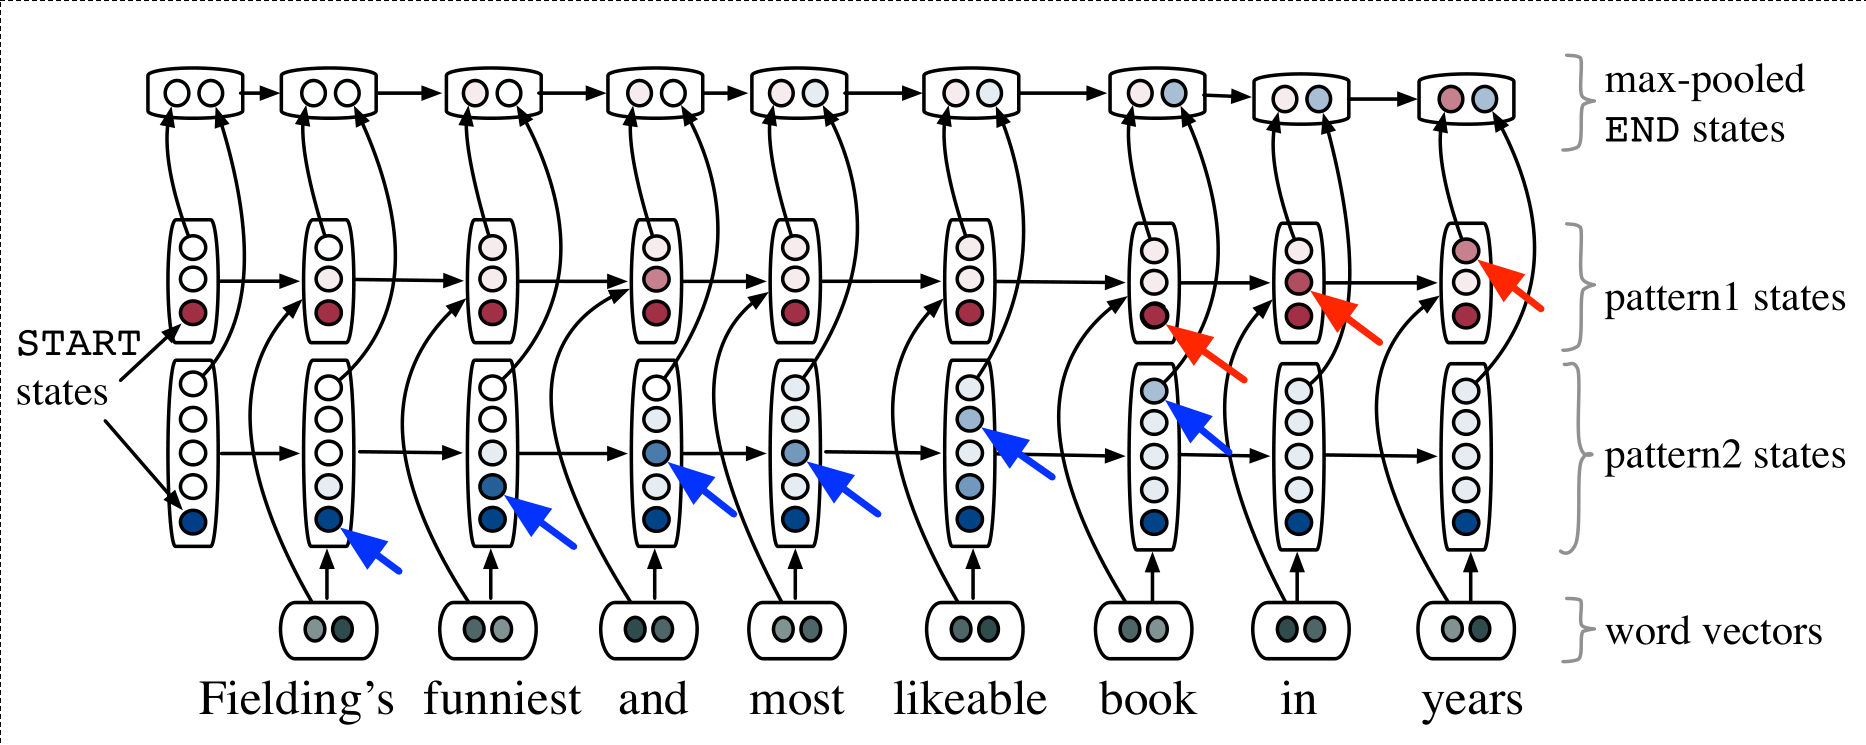
\includegraphics[trim={0.5cm 0.5cm 0.5cm 0.5cm},clip,width=14cm]{images/sopa_computational_graph.png}
  \caption{Schematic visualizing the SoPa model framework with two constituent WFSAs highlighted in blue and red; figure taken from \citet{schwartz2018sopa}}
  \label{fig:sopa}
\end{figure}

\paragraph{Hyperparameters:} Creating and training the SoPa model requires both commonly used and special hyperparameters. Commonly used hyperparameters include the learning rate, neuron dropout and word dropout. A special hyperparameter in the SoPa model is the pattern hyperparameter and it contains information on the number of patterns or WFSAs allowed, as well as the lengths of the patterns or the number of states in the WFSAs. This hyperparameter is encoded as a string with the following syntax: \texttt{Length$_{1}$-Count$_{1}$\_$\dots$\_Length$_{n}$-Count$_{n}$}. An example of this hyperparameter could be \texttt{3-5\_4-10\_5-15}, which would signify 5 patterns of length 3, 10 patterns of length 4 and 15 patterns of length 5.

\paragraph{Explainability:} In their study, \citet{schwartz2018sopa} describe simple methods of \textit{``interpreting''} the SoPa model. One method involves the usage of back-pointers during the Viterbi computation to determine the patterns and substrings in a document which contributed the highest pattern scores. Another method involves zeroing out the corresponding patterns or WFSAs via the occlusion sensitivity method to determine which pattern had the greatest impact on each classification decision. It is worth noting that the usage of \textit{interpretation} in \citet{schwartz2018sopa} is likely inconsistent with our definitions presented in Section \ref{section:xai}. Given the common terminology misuse described in Section \ref{section:xai-terminology}, it is more accurate to present the aforementioned \textit{``interpretability''} method as an explainability method. We analyze the explainability-related features of SoPa in greater detail in Sections \ref{section:sopa-transparency} and \ref{section:sopa-explainability}. 

\subsection{Transparency of SoPa}

\label{section:sopa-transparency}

Since we expounded on XAI in Section \ref{section:xai} and made a case for viewing ML models from the lens of XAI, it would only make sense to extend the same standards to the SoPa model. Based on the arguments made by \citet{arrieta2020explainable}, we can classify the SoPa model as a black-box model since it closely resembles RNNs and CNNs; and a strong case has already been made in their study regarding the black-box natures of both RNNs and CNNs. Naturally, this would imply that post-hoc explainability methods are required to explain the SoPa model. 

\subsection{Post-hoc explainability methods}

\label{section:sopa-explainability}

Using the post-hoc explainability taxonomies described in Section \ref{section:xai-techniques}, we can correspondingly classify the explainability methods presented in \citet{schwartz2018sopa} using terminology consistent with XAI research. The first explainability method uses individual text samples to determine the highest scoring substrings in documents; as well as the patterns or WFSAs corresponding to them. Since this analysis is conducted at an individual document level and is never synthesized to a more global context, we would classify this under the local explanations explainability method. The next technique involves an occlusion or sensitivity analysis over all patterns and documents to determine which pattern had the greatest impact for each class. Since this involves systematic perturbation to determine the importance of pattern features, we would classify this method as a feature relevance explainability method.

Section \ref{section:xai-metrics} describes basic guidelines that could help elucidate what constitutes a good explanation; namely that a good explanation should be constrictive, provide causal links and be selective. We attempt to apply these guidelines with the aforementioned explainability techniques presented in SoPa. For the constrictive quality, it is likely that the explainability methods do not meet this criterion since they only highlight individual features that were important for SoPa, and do not necessarily go into detail regarding why these features superseded adjacent features. Next, the explainability methods likely do not fulfill the criterion of providing causal links; since they generally provide explanations by aggregating (ultimately) probabilistic quantities inside SoPa. Finally in contrast, the explainability methods likely pass the criterion of being selective since they only provide the most important features for an explanation. 

%%% Local Variables: 
%%% mode: latex
%%% TeX-master: "main"
%%% End: 

% LocalWords:  XAI Interpretability understandability simulatable decomposable
% LocalWords:  algorithmically Simulatability Decomposability regressors NLP
% LocalWords:  Explainability interpretability explainability subspaces Shapley
% LocalWords:  Interpretable SHAP Automata FSAs WFSAs pdfs tradeoff pdf ste MLP
% LocalWords:  quantized STE's STEs Semiring semiring Semirings semirings WFSA
% LocalWords:  substring Viterbi CNNs LSTM automata substrings Perceptron RNNs
% LocalWords:  Hyperparameters hyperparameters tterns hyperparameter
